%==============================================================================
%  MATH 231 -- Linear Algebra I (Queens College, Fall 2026)
%  MATRIX UNIT, PART 4 -- Area, and the Rotation Matrix
%
%  Section numbering runs CONTINUOUSLY across the parts of the matrix unit;
%  see Part 2's header for the full map.  This part is Sections 22-25, hence
%  \setcounter{section}{21}.
%
%  STATUS: complete.  Sections 22-25.  Written from the plan in
%  plan/MATH231_remaining_units_plan.tex (2026-10-25).
%
%  AUDIENCE: distributed to students.  No instructor-facing apparatus.
%
%  WHAT THE INSTRUCTOR SPECIFIED, AND WHERE IT IS.
%   - Properties of the 2x2 determinant, including det(aA) = a^2 det A and
%     det(AB) = det A det B: Sec. 22, each with a one-line proof.
%   - The area derivation, exactly as specified: a_1 = [a,c], a_2 = [b,d];
%     base ||a_1||, height ||a_2|| sin(theta); Area^2 expanded; Area =
%     |ad - bc| = |det A|: Sec. 23.1-23.4.
%   - The rotation matrix from a parameterization of the unit circle by
%     angle; R_theta' R_theta = I for all theta; det R_theta = 1 for all
%     theta: Sec. 24.1-24.5.
%   - Rotations in R^3, and rotation with respect to a plane: Sec. 25.
%
%  DECISIONS CARRIED FROM THE PLAN.
%
%   D10. The angle-addition formulas appear in no earlier course document.
%        Sec. 24.4 states them, and shows the rotation matrix is equivalent
%        to them (R_theta applied to [cos t, sin t] IS the pair of formulas).
%        Sec. 24.2 avoids needing them for e_2 by turning [cos th, sin th] a
%        quarter-turn with J (Sec. 19.1) instead.
%
%   D11. R_alpha R_beta = R_(alpha+beta) is read as "rotate by beta, then by
%        alpha" via M1, as in Sec. 15.4.
%
%   LINEARITY OF ROTATION (Sec. 24.2) is argued geometrically -- a rotation
%   carries the parallelogram of x and y to the parallelogram of their
%   images -- not proved from axioms.  That is the honest level for this
%   course.
%
%   3x3 DETERMINANTS are not defined until Part 7, so Sec. 25 says the R^3
%   rotations are orthogonal and defers "det = 1" to Sec. 39.3.
%
%  Compile with pdflatex or tectonic (standard TeX Live packages only; uses
%  tikz).
%==============================================================================
\documentclass[11pt]{article}

\usepackage[margin=1in]{geometry}
\usepackage{amsmath,amssymb,amsthm}
\usepackage[dvipsnames]{xcolor}
\usepackage{enumitem}
\usepackage{booktabs}
\usepackage{array}
\usepackage[hidelinks]{hyperref}
\usepackage{titlesec}
\usepackage{needspace}
\usepackage{tikz}
\usetikzlibrary{arrows.meta}

%------------------------------------------------------------------ style ----
\titleformat{\section}{\large\bfseries\sffamily}{\thesection.}{0.6em}{}
\titleformat{\subsection}{\normalsize\bfseries\sffamily}{\thesubsection.}{0.5em}{}
\titlespacing*{\section}{0pt}{14pt}{6pt}
\setlength{\emergencystretch}{3em}

\theoremstyle{plain}
\newtheorem{thm}{Theorem}[section]
\newtheorem{lem}[thm]{Lemma}
\newtheorem{cor}[thm]{Corollary}

\theoremstyle{definition}
\newtheorem{defn}{Definition}[section]
\newtheorem{ex}{Example}[section]
\theoremstyle{remark}
\newtheorem*{rmk}{Remark}
\newtheorem*{warn}{A common confusion}

\newcommand{\lookahead}{\par\smallskip\noindent
  \textbf{\sffamily\textcolor{RoyalBlue}{Looking ahead.}}\ \ignorespaces}
\newcommand{\lookback}[1][the vector unit]{\par\smallskip\noindent
  \textbf{\sffamily\textcolor{ForestGreen}{From #1.}}\ \ignorespaces}

%--------------------------------------------------------------- notation ----
\newcommand{\R}{\mathbb{R}}
\newcommand{\vc}[1]{\mathbf{#1}}
\newcommand{\mt}[1]{\mathbf{#1}}
\newcommand{\norm}[1]{\lVert #1\rVert}
\newcommand{\T}{^{\mathsf{T}}}
\newcommand{\smat}[1]{\left[\begin{smallmatrix}#1\end{smallmatrix}\right]}
\DeclareMathOperator{\spanop}{span}
\DeclareMathOperator{\diagop}{diag}
\DeclareMathOperator{\rank}{rank}

%------------------------------------------------------------- tikz helpers --
\tikzset{
  vecarr/.style   = {-{Stealth[length=2.6mm,width=2.0mm]},very thick},
  thinarr/.style  = {-{Stealth[length=2.2mm,width=1.7mm]},thick},
  axisline/.style = {->,gray!75,thin}
}

\title{\vspace{-1.2cm}\textbf{\sffamily MATH 231 -- Linear Algebra I}\\[4pt]
       {\large\sffamily The Matrix Unit, Part 4 \textbullet\ Area, and the
        Rotation Matrix}\\[2pt]
       {\normalsize\sffamily Kiely Hall 326 \textbullet\
        Instructor: Kevin Bedoya}}
\author{}
\date{}

\begin{document}
\setcounter{section}{21}  % this part opens at Section 22; see the header note
\maketitle
\vspace{-1.6cm}

\noindent\textbf{About this document.} This is Part 4 of the matrix unit,
Sections 22--25. Section numbers run continuously through the unit (Part 2's
opening table lists them all). References into the vector unit always name it.

\medskip
\noindent\textbf{Assumed.} The $2\times2$ determinant and its meaning (\S14);
the gallery of motions and the two families of $2\times2$ orthogonal matrices
(\S16--\S21); the quarter-turn $\mt{J}$ (\S19.1); the laws M1--M6 (\S8.4). From
the vector unit: the angle between two vectors (\S10.3), the dot product formula
$\vc{u}\cdot\vc{v}=\norm{\vc{u}}\norm{\vc{v}}\cos\theta$ (\S11.3), and the
Cauchy--Schwarz inequality (\S13).

\medskip
\noindent\textbf{What you should be able to do afterwards.} Use the properties
of the $2\times2$ determinant to compute determinants of scaled, transposed and
multiplied matrices without multiplying them out; derive the area of a
parallelogram from base and height and show it equals $|\det\mt{A}|$; derive the
rotation matrix $\mt{R}_\theta$ from the unit circle, and show it is orthogonal
with determinant $1$; compose and undo rotations; and write the matrices of
rotations of $\R^{3}$ about the coordinate axes.

%==============================================================================
\section{Properties of the \texorpdfstring{$2\times2$}{2x2} determinant}
%==============================================================================
Throughout this section
\[
  \mt{A}=\begin{bmatrix}a&b\\c&d\end{bmatrix},\qquad
  \mt{B}=\begin{bmatrix}e&f\\g&h\end{bmatrix},\qquad
  \det\mt{A}=ad-bc,\qquad \det\mt{B}=eh-fg .
\]
Each property comes with a one-line proof by computation, and each is worth
reading against the gallery of Part 3. The same properties hold for
$n\times n$ matrices, in the form Part 7 gives them.

%------------------------------------------------------------------------------
\subsection{The identity and the transpose}
%------------------------------------------------------------------------------
\textbf{P1.} $\det\mt{I}=1\cdot1-0\cdot0=1$. The identity moves nothing, so
every area is unchanged.

\textbf{P2.} $\det\mt{A}\T=\det\mt{A}$. Indeed
$\mt{A}\T=\begin{bmatrix}a&c\\b&d\end{bmatrix}$ has determinant $ad-cb$. This
is the observation of \S12.4 that the same number tests the rows and the
columns. Every statement below about columns is therefore true of rows too.

%------------------------------------------------------------------------------
\subsection{Scaling}
%------------------------------------------------------------------------------
\textbf{P3.} $\det(\alpha\mt{A})=\alpha^{2}\det\mt{A}$. Indeed
$(\alpha a)(\alpha d)-(\alpha b)(\alpha c)=\alpha^{2}(ad-bc)$.

\noindent Not $\alpha\det\mt{A}$: scaling the matrix scales \emph{both}
columns, so both sides of the parallelogram, and the area picks up the factor
twice. With $\mt{A}=\mt{I}$ this is the uniform scaling of \S16.1:
$\det(\alpha\mt{I})=\alpha^{2}$.

%------------------------------------------------------------------------------
\subsection{The columns}
%------------------------------------------------------------------------------
\textbf{P4.} \emph{Swapping the two columns changes the sign.}
$\det\begin{bmatrix}b&a\\d&c\end{bmatrix}=bc-ad=-\det\mt{A}$. By P2, the same
holds for swapping the rows. (This is the pair of matrices in the middle and left
pictures of \S14.4.)

\textbf{P5.} \emph{The determinant is linear in each column separately.} Write
$\det[\,\vc{u}\ \ \vc{w}\,]$ for the determinant of the matrix with columns
$\vc{u}$ and $\vc{w}$. Then
\[
  \det[\,\alpha\vc{u}+\beta\vc{v}\ \ \vc{w}\,]
  =\alpha\det[\,\vc{u}\ \ \vc{w}\,]+\beta\det[\,\vc{v}\ \ \vc{w}\,] ,
\]
since
$(\alpha u_1+\beta v_1)w_2-(\alpha u_2+\beta v_2)w_1
 =\alpha(u_1w_2-u_2w_1)+\beta(v_1w_2-v_2w_1)$. Likewise in the second column.

\begin{warn}[Linear in each column is not linear in the matrix]
P5 holds one column fixed. The determinant of a sum of matrices is \emph{not}
the sum of the determinants: $\det(\mt{I}+\mt{I})=\det(2\mt{I})=4$, while
$\det\mt{I}+\det\mt{I}=2$.
\end{warn}

\textbf{P6.} \emph{Two parallel columns give zero.} If $\vc{w}=k\vc{u}$ then
$u_1(ku_2)-u_2(ku_1)=0$. In particular two equal columns give zero.

\textbf{P7.} \emph{Adding a multiple of one column to the other changes
nothing.} By P5 and P6,
\[
  \det[\,\vc{a}_1\ \ \vc{a}_2+k\vc{a}_1\,]
  =\det[\,\vc{a}_1\ \ \vc{a}_2\,]+k\det[\,\vc{a}_1\ \ \vc{a}_1\,]
  =\det\mt{A}+0 .
\]
Geometrically, $\vc{a}_2$ slides parallel to $\vc{a}_1$, which is a shear of the
parallelogram (\S18): the base and the height stay the same, so the area does
too.

%------------------------------------------------------------------------------
\subsection{Products}
%------------------------------------------------------------------------------
\textbf{P8.} $\det(\mt{A}\mt{B})=\det\mt{A}\,\det\mt{B}$. The product is
$\mt{A}\mt{B}=\begin{bmatrix}ae+bg&af+bh\\ce+dg&cf+dh\end{bmatrix}$, so
\[
  \det(\mt{A}\mt{B})=(ae+bg)(cf+dh)-(af+bh)(ce+dg) .
\]
Expanding gives eight terms. The four $aecf-afce$ and $bgdh-bhdg$ cancel in
pairs, and the rest regroup:
\[
  aedh+bgcf-afdg-bhce
  =ad(eh-fg)-bc(eh-fg)
  =(ad-bc)(eh-fg) .
\]

\noindent Two consequences are worth stating. First, by \S15.4 the product is
``first $\mt{B}$, then $\mt{A}$'', and P8 says the area factors multiply: $\mt{B}$
scales areas by $|\det\mt{B}|$, then $\mt{A}$ by $|\det\mt{A}|$. Second,
$\det(\mt{A}\mt{B})=\det(\mt{B}\mt{A})$, because both equal the product of two
numbers. The matrices $\mt{A}\mt{B}$ and $\mt{B}\mt{A}$ are usually different
(\S8.4), and their determinants are always equal, like their traces (\S9.3).

%------------------------------------------------------------------------------
\subsection{Special matrices}
%------------------------------------------------------------------------------
\textbf{P9.} \emph{Triangular and diagonal.}
$\det\begin{bmatrix}a&b\\0&d\end{bmatrix}=ad$,
$\det\begin{bmatrix}a&0\\c&d\end{bmatrix}=ad$, and
$\det\diagop(s_1,s_2)=s_1s_2$: the product of the diagonal.

\textbf{P10.} \emph{Orthogonal.} If $\mt{Q}\T\mt{Q}=\mt{I}$ then by P8, P2 and
P1, $(\det\mt{Q})^{2}=\det\mt{Q}\T\det\mt{Q}=\det(\mt{Q}\T\mt{Q})=\det\mt{I}=1$,
so $\det\mt{Q}=\pm1$. This is what \S21.2 found by listing every case, now
obtained without the list.

\textbf{P11.} $\det\mt{A}\neq0$ exactly when $\rank\mt{A}=2$ (\S14.2).

%------------------------------------------------------------------------------
\subsection{The gallery, by determinant}
%------------------------------------------------------------------------------
\begin{center}
\renewcommand{\arraystretch}{1.4}
\begin{tabular}{@{}l c l@{}}
\toprule
\textbf{Motion} & $\det$ & \textbf{Which property explains it} \\
\midrule
uniform scaling $\alpha\mt{I}$ & $\alpha^{2}$ & P3 with $\mt{A}=\mt{I}$ \\
scaling the axes, $\diagop(s_1,s_2)$ & $s_1s_2$ & P9 \\
shear $\smat{1&k\\0&1}$ & $1$ & P9, or P7 applied to $\mt{I}$ \\
rotation & $1$ & P10, the $+1$ family \\
reflection & $-1$ & P10, the $-1$ family; or P4 applied to $\mt{I}$ for $\smat{0&1\\1&0}$ \\
projection $\diagop(1,0)$ & $0$ & P9, or P11 (rank $1$) \\
\bottomrule
\end{tabular}
\end{center}

%==============================================================================
\section{The determinant is an area}
%==============================================================================
\S14.3 claimed that the parallelogram with sides $\vc{a}_1$ and $\vc{a}_2$ has
area $|\det\mt{A}|$. This section proves it, starting from the oldest area
formula there is.

%------------------------------------------------------------------------------
\subsection{Base times height}
%------------------------------------------------------------------------------
Let the columns of $\mt{A}=\begin{bmatrix}a&b\\c&d\end{bmatrix}$ be
\[
  \vc{a}_1=\begin{bmatrix}a\\c\end{bmatrix},
  \qquad
  \vc{a}_2=\begin{bmatrix}b\\d\end{bmatrix},
\]
linearly independent, so that neither is zero and they are not parallel. Let
$\theta$ be the angle between them (the vector unit, \S10.3); then
$0<\theta<\pi$. The area of a parallelogram is its base times its height.
\begin{itemize}[leftmargin=1.4em,itemsep=3pt]
  \item Take the side $\vc{a}_1$ as the base. Its length is $\norm{\vc{a}_1}$.
  \item The height is the distance from the tip of $\vc{a}_2$ to the line
        through $\vc{a}_1$. It is the side opposite the angle $\theta$ in a right
        triangle with hypotenuse $\norm{\vc{a}_2}$, so it is
        $\norm{\vc{a}_2}\sin\theta$.
\end{itemize}
So
\[
  \text{Area}=\norm{\vc{a}_1}\,\norm{\vc{a}_2}\,\sin\theta .
\]

\begin{center}
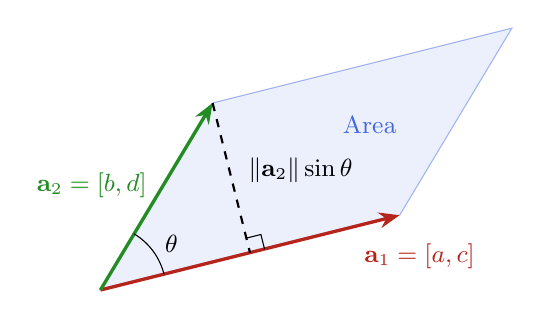
\begin{tikzpicture}[scale=0.95]
  \fill[RoyalBlue!10] (0,0) -- (4,1) -- (5.5,3.5) -- (1.5,2.5) -- cycle;
  \draw[RoyalBlue!50] (4,1) -- (5.5,3.5) -- (1.5,2.5);
  \draw[vecarr,BrickRed] (0,0) -- (4,1);
  \draw[vecarr,ForestGreen] (0,0) -- (1.5,2.5);
  \draw[dashed,thick] (1.5,2.5) -- (2,0.5);
  % right-angle mark at the foot (2,0.5) of the height
  \draw (2.194,0.5485) -- (2.1455,0.7425) -- (1.9515,0.694);
  \draw (0.85,0.2125) arc[start angle=14.04,end angle=59.04,radius=0.875];
  \node[font=\small] at (0.95,0.62) {$\theta$};
  \node[below right,font=\small,BrickRed] at (3.4,0.75) {$\vc{a}_1=[a,c]$};
  \node[left,font=\small,ForestGreen] at (0.75,1.4) {$\vc{a}_2=[b,d]$};
  \node[right,font=\small] at (1.85,1.6) {$\norm{\vc{a}_2}\sin\theta$};
  \node[font=\small,RoyalBlue] at (3.6,2.2) {Area};
\end{tikzpicture}
\end{center}

%------------------------------------------------------------------------------
\subsection{Getting rid of the sine}
%------------------------------------------------------------------------------
The sine is the awkward part: the entries $a,b,c,d$ do not obviously know
anything about $\sin\theta$. They do know about $\cos\theta$, through the dot
product. So square the area, and trade $\sin^{2}\theta$ for
$1-\cos^{2}\theta$:
\[
  \text{Area}^{2}
  =\norm{\vc{a}_1}^{2}\norm{\vc{a}_2}^{2}\sin^{2}\theta
  =\norm{\vc{a}_1}^{2}\norm{\vc{a}_2}^{2}\bigl(1-\cos^{2}\theta\bigr)
  =\norm{\vc{a}_1}^{2}\norm{\vc{a}_2}^{2}
   -\bigl(\norm{\vc{a}_1}\norm{\vc{a}_2}\cos\theta\bigr)^{2} .
\]
\lookback The last bracket is the dot product:
$\vc{a}_1\cdot\vc{a}_2=\norm{\vc{a}_1}\norm{\vc{a}_2}\cos\theta$ (\S11.3). So
\[
  \text{Area}^{2}=\norm{\vc{a}_1}^{2}\norm{\vc{a}_2}^{2}-(\vc{a}_1\cdot\vc{a}_2)^{2},
\]
and every quantity on the right is computed from the entries alone.

%------------------------------------------------------------------------------
\subsection{In coordinates}
%------------------------------------------------------------------------------
With $\norm{\vc{a}_1}^{2}=a^{2}+c^{2}$, $\norm{\vc{a}_2}^{2}=b^{2}+d^{2}$ and
$\vc{a}_1\cdot\vc{a}_2=ab+cd$,
\[
  \text{Area}^{2}=(a^{2}+c^{2})(b^{2}+d^{2})-(ab+cd)^{2} .
\]
Expand both products:
\[
  (a^{2}b^{2}+a^{2}d^{2}+c^{2}b^{2}+c^{2}d^{2})
  -(a^{2}b^{2}+2abcd+c^{2}d^{2})
  =a^{2}d^{2}-2abcd+b^{2}c^{2}
  =(ad-bc)^{2} .
\]

%------------------------------------------------------------------------------
\subsection{The result}
%------------------------------------------------------------------------------
Take square roots. The area is not negative, and neither is $\sin\theta$ for
$0\le\theta\le\pi$, so
\[
  \text{Area}=\sqrt{(ad-bc)^{2}}=|ad-bc| .
\]

\begin{thm}
\label{thm:area}
The parallelogram with sides $\vc{a}_1=[\,a,c\,]$ and $\vc{a}_2=[\,b,d\,]$ has
area
\[
  \boxed{\;\text{Area}=|ad-bc|=|\det\mt{A}|\;}
  \qquad\text{where }\mt{A}=\begin{bmatrix}a&b\\c&d\end{bmatrix}.
\]
\end{thm}

\noindent The formula also covers the case set aside at the start. If
$\vc{a}_1$ and $\vc{a}_2$ are parallel, the parallelogram is flat, its area is
$0$, and so is $\det\mt{A}$ (P6).

\begin{ex}
For $\vc{a}_1=[\,3,0\,]$ and $\vc{a}_2=[\,1,2\,]$, the base lies along the
$x$-axis with length $3$ and the height is $2$, so the area is $6$; and
$\det\begin{bmatrix}3&1\\0&2\end{bmatrix}=6$. For the matrix
$\begin{bmatrix}2&1\\1&2\end{bmatrix}$ of \S13.4, base times height is less
obvious, but the theorem gives $|4-1|=3$ at once.
\end{ex}

%------------------------------------------------------------------------------
\subsection{What else the identity says}
%------------------------------------------------------------------------------
\textbf{Cauchy--Schwarz, with the gap measured.} The middle line of \S23.2 can
be read as
\[
  \norm{\vc{a}_1}^{2}\norm{\vc{a}_2}^{2}-(\vc{a}_1\cdot\vc{a}_2)^{2}
  =(\det\mt{A})^{2}\;\ge\;0 .
\]
That is the Cauchy--Schwarz inequality
$|\vc{a}_1\cdot\vc{a}_2|\le\norm{\vc{a}_1}\norm{\vc{a}_2}$ of the vector unit's
\S13, in $\R^{2}$, with the amount by which it is strict given exactly. Equality
holds exactly when $\det\mt{A}=0$, that is, when the vectors are parallel, which
is the equality case found in the vector unit's \S13.

\textbf{A second formula for the area.} The same quantity is the determinant
of $\mt{A}\T\mt{A}$:
\[
  \mt{A}\T\mt{A}=\begin{bmatrix}\norm{\vc{a}_1}^{2}&\vc{a}_1\cdot\vc{a}_2\\
                 \vc{a}_1\cdot\vc{a}_2&\norm{\vc{a}_2}^{2}\end{bmatrix},
  \qquad
  \det(\mt{A}\T\mt{A})=\norm{\vc{a}_1}^{2}\norm{\vc{a}_2}^{2}-(\vc{a}_1\cdot\vc{a}_2)^{2}
  =\text{Area}^{2},
\]
in agreement with P8 and P2: $\det(\mt{A}\T\mt{A})=(\det\mt{A})^{2}$.

%------------------------------------------------------------------------------
\subsection{Every area, not just one}
%------------------------------------------------------------------------------
A square of the grid with corner $\vc{p}$ and side $h$ is spanned by $h\vc{e}_1$
and $h\vc{e}_2$. By linearity, $\mt{A}$ sends it to the parallelogram with
corner $\mt{A}\vc{p}$ spanned by $h\vc{a}_1$ and $h\vc{a}_2$, whose area by the
theorem and P3 is $|\det[\,h\vc{a}_1\ h\vc{a}_2\,]|=h^{2}|\det\mt{A}|$. Every
small square has its area multiplied by the same factor $|\det\mt{A}|$. Any
region can be approximated by small squares, and its image by the corresponding
parallelograms, so
\[
  \text{area of the image of a region}=|\det\mt{A}|\times\text{area of the region}.
\]
Read with this, P8 says that doing $\mt{B}$ and then $\mt{A}$ scales every area
by $|\det\mt{B}|$ and then by $|\det\mt{A}|$. That is why the determinant of a
product is the product of the determinants.

%==============================================================================
\section{The rotation matrix}
%==============================================================================

%------------------------------------------------------------------------------
\subsection{The unit circle, by angle}
%------------------------------------------------------------------------------
Every point of the unit circle can be written
\[
  [\,\cos t,\ \sin t\,]
\]
for an angle $t$ measured counterclockwise from the positive $x$-axis; that is
what cosine and sine \emph{are}. As $t$ runs from $0$ to $2\pi$ the point goes
once around. The standard basis vectors sit at two particular angles:
$\vc{e}_1=[\,\cos0,\sin0\,]$ at $t=0$, and
$\vc{e}_2=[\,\cos\frac{\pi}{2},\sin\frac{\pi}{2}\,]$ at $t=\frac{\pi}{2}$.

%------------------------------------------------------------------------------
\subsection{Rotating by \texorpdfstring{$\theta$}{theta}}
%------------------------------------------------------------------------------
Rotation by $\theta$ about the origin keeps every point at the same distance
from the origin and adds $\theta$ to its angle. On the unit circle,
\[
  [\,\cos t,\ \sin t\,]\;\longmapsto\;[\,\cos(t+\theta),\ \sin(t+\theta)\,].
\]

\noindent It is linear. A rotation moves the plane rigidly, so it carries the
parallelogram with sides $\vc{x}$ and $\vc{y}$ to the parallelogram with sides
the rotated $\vc{x}$ and the rotated $\vc{y}$. The diagonal goes with it, so the
image of $\vc{x}+\vc{y}$ is the sum of the images. Stretching $\vc{x}$ before
rotating is the same as stretching after. So \S13.3 applies: the matrix is
determined by where $\vc{e}_1$ and $\vc{e}_2$ go.

\begin{itemize}[leftmargin=1.4em,itemsep=4pt]
  \item $\vc{e}_1$, at angle $0$, goes to the point at angle $\theta$:
        \[\vc{e}_1\longmapsto[\,\cos\theta,\ \sin\theta\,].\]
  \item $\vc{e}_2$, at angle $\frac{\pi}{2}$, goes to the point at angle
        $\theta+\frac{\pi}{2}$. That point is the previous one turned a further
        quarter-turn, and \S19.1 says a quarter-turn sends $[\,x,y\,]$ to
        $[\,-y,x\,]$:
        \[\vc{e}_2\longmapsto
          \mt{J}\begin{bmatrix}\cos\theta\\\sin\theta\end{bmatrix}
          =[\,-\sin\theta,\ \cos\theta\,].\]
\end{itemize}

\begin{defn}[Rotation matrix]
The matrix of the counterclockwise rotation of $\R^{2}$ by the angle $\theta$
is
\[
  \boxed{\;\mt{R}_\theta=\begin{bmatrix}\cos\theta&-\sin\theta\\
                                       \sin\theta&\cos\theta\end{bmatrix}.\;}
\]
\end{defn}

\begin{center}
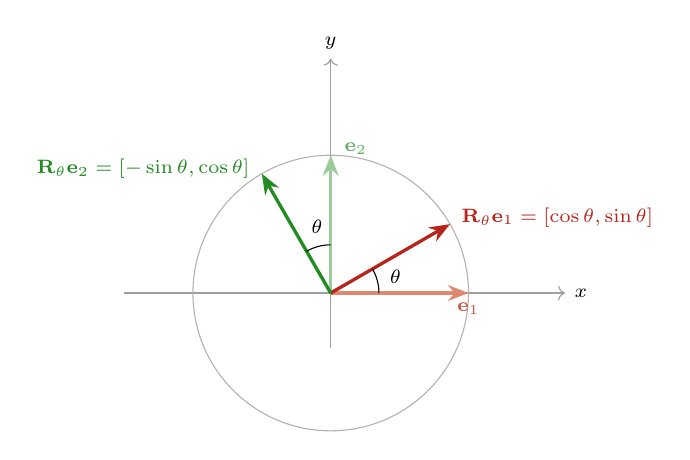
\begin{tikzpicture}[scale=1.75]
  \draw[axisline] (-1.5,0) -- (1.7,0) node[right,font=\scriptsize,black]{$x$};
  \draw[axisline] (0,-0.4) -- (0,1.7) node[above,font=\scriptsize,black]{$y$};
  \draw[gray!60] (0,0) circle (1);
  \draw[vecarr,BrickRed!45] (0,0) -- (1,0);
  \draw[vecarr,ForestGreen!45] (0,0) -- (0,1);
  \draw[vecarr,BrickRed] (0,0) -- (0.866,0.5);
  \draw[vecarr,ForestGreen] (0,0) -- (-0.5,0.866);
  \draw[thin] (0.35,0) arc[start angle=0,end angle=30,radius=0.35];
  \node[font=\scriptsize] at (0.47,0.12) {$\theta$};
  \draw[thin] (0,0.35) arc[start angle=90,end angle=120,radius=0.35];
  \node[font=\scriptsize] at (-0.1,0.48) {$\theta$};
  \node[below,font=\scriptsize,BrickRed!70] at (1,0) {$\vc{e}_1$};
  \node[right,font=\scriptsize,ForestGreen!70] at (0.03,1.05) {$\vc{e}_2$};
  \node[right,font=\scriptsize,BrickRed] at (0.88,0.55)
       {$\mt{R}_\theta\vc{e}_1=[\cos\theta,\sin\theta]$};
  \node[left,font=\scriptsize,ForestGreen] at (-0.52,0.9)
       {$\mt{R}_\theta\vc{e}_2=[-\sin\theta,\cos\theta]$};
\end{tikzpicture}
\end{center}

%------------------------------------------------------------------------------
\subsection{Checks}
%------------------------------------------------------------------------------
\begin{ex}
\label{ex:rot}
\leavevmode
\begin{itemize}[leftmargin=1.4em,itemsep=3pt]
  \item $\theta=0$: $\mt{R}_0=\mt{I}$. No rotation.
  \item $\theta=\frac{\pi}{2}$: $\mt{R}_{\pi/2}=\begin{bmatrix}0&-1\\1&0\end{bmatrix}=\mt{J}$,
        the quarter-turn of \S19.1.
  \item $\theta=\pi$: $\mt{R}_\pi=-\mt{I}$, the half-turn.
  \item $\theta=\frac{\pi}{4}$: $\mt{R}_{\pi/4}=\frac{1}{\sqrt2}\begin{bmatrix}1&-1\\1&1\end{bmatrix}$,
        and it rotates $[\,2,1\,]$ to $\frac{1}{\sqrt2}[\,1,3\,]$. Both have
        length $\sqrt5$.
\end{itemize}
\end{ex}

%------------------------------------------------------------------------------
\subsection{Every point turns, and the angle-addition formulas}
%------------------------------------------------------------------------------
The matrix was built from two points. Linearity guarantees it rotates every
other point too, and it is instructive to watch that happen on the unit circle:
\[
  \mt{R}_\theta\begin{bmatrix}\cos t\\\sin t\end{bmatrix}
  =\begin{bmatrix}\cos\theta\cos t-\sin\theta\sin t\\
                  \sin\theta\cos t+\cos\theta\sin t\end{bmatrix} .
\]
Rotation should produce $[\,\cos(t+\theta),\sin(t+\theta)\,]$, and so the two
entries are the \textbf{angle-addition formulas}:
\[
  \cos(t+\theta)=\cos t\cos\theta-\sin t\sin\theta,
  \qquad
  \sin(t+\theta)=\sin t\cos\theta+\cos t\sin\theta .
\]
They are one statement about one matrix. Anyone who remembers $\mt{R}_\theta$
can recover them by multiplying it into $[\,\cos t,\sin t\,]$.

%------------------------------------------------------------------------------
\subsection{\texorpdfstring{$\mt{R}_\theta$}{R\_theta} is orthogonal, with determinant \texorpdfstring{$1$}{1}}
%------------------------------------------------------------------------------
\begin{thm}
\label{thm:rotorth}
For every angle $\theta$,
\[
  \mt{R}_\theta\T\mt{R}_\theta=\mt{I}
  \qquad\text{and}\qquad
  \det\mt{R}_\theta=1 .
\]
\end{thm}

\begin{proof}
Multiply out, using $\cos^{2}\theta+\sin^{2}\theta=1$:
\[
  \begin{aligned}
  \mt{R}_\theta\T\mt{R}_\theta
  &=\begin{bmatrix}\cos\theta&\sin\theta\\-\sin\theta&\cos\theta\end{bmatrix}
   \begin{bmatrix}\cos\theta&-\sin\theta\\\sin\theta&\cos\theta\end{bmatrix}\\
  &=\begin{bmatrix}\cos^{2}\theta+\sin^{2}\theta & -\cos\theta\sin\theta+\sin\theta\cos\theta\\
                  -\sin\theta\cos\theta+\cos\theta\sin\theta & \sin^{2}\theta+\cos^{2}\theta\end{bmatrix}
  =\mt{I}.
  \end{aligned}
\]
And $\det\mt{R}_\theta=\cos\theta\cdot\cos\theta-(-\sin\theta)\sin\theta
=\cos^{2}\theta+\sin^{2}\theta=1$.
\end{proof}

\noindent So every rotation preserves lengths and angles (\S20.5) and
orientation and area ($\det=1$). And $\mt{R}_\theta$ is exactly the first family
of \S21.2, $\begin{bmatrix}a&-c\\c&a\end{bmatrix}$, with $a=\cos\theta$ and
$c=\sin\theta$. Conversely every member of that family is a rotation, because a
point $[\,a,c\,]$ on the unit circle is $[\,\cos\theta,\sin\theta\,]$ for some
$\theta$. In the plane:
\[
  \text{orthogonal with }\det=+1
  \quad\Longleftrightarrow\quad
  \text{a rotation }\mt{R}_\theta .
\]

%------------------------------------------------------------------------------
\subsection{Composing and undoing rotations}
%------------------------------------------------------------------------------
Rotating by $\beta$ and then by $\alpha$ is, by \S15.4, the product
$\mt{R}_\alpha\mt{R}_\beta$, and geometrically it is a rotation by
$\alpha+\beta$. The angle-addition formulas confirm it entry by entry:
\[
  \mt{R}_\alpha\mt{R}_\beta
  =\begin{bmatrix}\cos\alpha\cos\beta-\sin\alpha\sin\beta & -(\cos\alpha\sin\beta+\sin\alpha\cos\beta)\\
                  \sin\alpha\cos\beta+\cos\alpha\sin\beta & \cos\alpha\cos\beta-\sin\alpha\sin\beta\end{bmatrix}
  =\mt{R}_{\alpha+\beta}.
\]
Since $\alpha+\beta=\beta+\alpha$, it follows that
$\mt{R}_\alpha\mt{R}_\beta=\mt{R}_\beta\mt{R}_\alpha$: rotations of the plane
commute, even though matrices in general do not.

To undo a rotation by $\theta$, rotate by $-\theta$. Since cosine is even and
sine is odd,
\[
  \mt{R}_{-\theta}
  =\begin{bmatrix}\cos\theta&\sin\theta\\-\sin\theta&\cos\theta\end{bmatrix}
  =\mt{R}_\theta\T,
  \qquad
  \mt{R}_\theta\T\mt{R}_\theta=\mt{R}_{-\theta}\mt{R}_\theta=\mt{R}_0=\mt{I},
\]
which is Theorem~\ref{thm:rotorth} again, read geometrically: \emph{the
transpose of a rotation is the rotation back.}

%------------------------------------------------------------------------------
\subsection{Reflections, by angle}
%------------------------------------------------------------------------------
The second family of \S21.2, with $a=\cos\theta$ and $c=\sin\theta$, is
\[
  \mt{F}_\theta=\begin{bmatrix}\cos\theta&\sin\theta\\\sin\theta&-\cos\theta\end{bmatrix}
  =\mt{R}_\theta\,\diagop(1,-1).
\]
So $\mt{F}_\theta$ means ``reflect across the $x$-axis, then rotate by
$\theta$''. \S21.3 showed it fixes $[\,1+\cos\theta,\sin\theta\,]$. With the
half-angle identities $1+\cos\theta=2\cos^{2}\frac{\theta}{2}$ and
$\sin\theta=2\sin\frac{\theta}{2}\cos\frac{\theta}{2}$, that vector is
$2\cos\frac{\theta}{2}\,[\,\cos\frac{\theta}{2},\sin\frac{\theta}{2}\,]$. So
$\mt{F}_\theta$ is the reflection across the line through the origin at angle
$\theta/2$. Check: $\mt{F}_0=\diagop(1,-1)$ reflects across the $x$-axis (angle
$0$), and $\mt{F}_{\pi/2}=\begin{bmatrix}0&1\\1&0\end{bmatrix}$ across $y=x$
(angle $\pi/4$).

\begin{rmk}[Complex numbers]
Multiplying $x+iy$ by $\cos\theta+i\sin\theta$ gives
$(x\cos\theta-y\sin\theta)+i(x\sin\theta+y\cos\theta)$, the same arithmetic as
$\mt{R}_\theta[\,x,y\,]$. Multiplying by a complex number of modulus $1$ is a
rotation of the complex plane, and $\mt{R}_\theta$ is its matrix. The rule
$\mt{R}_\alpha\mt{R}_\beta=\mt{R}_{\alpha+\beta}$ is the rule that the angles of
complex numbers add when they are multiplied.
\end{rmk}

%==============================================================================
\section{Rotations in \texorpdfstring{$\R^{3}$}{R3}}
%==============================================================================

%------------------------------------------------------------------------------
\subsection{About the \texorpdfstring{$z$}{z}-axis}
%------------------------------------------------------------------------------
In space, a rotation turns about an \emph{axis}, a line through the origin that
stays fixed. The simplest axis is the $z$-axis. A rotation about it by $\theta$
turns the $xy$-plane exactly as $\mt{R}_\theta$ turns the plane and leaves
heights alone:
\[
  \vc{e}_1\mapsto[\,\cos\theta,\ \sin\theta,\ 0\,],\qquad
  \vc{e}_2\mapsto[\,-\sin\theta,\ \cos\theta,\ 0\,],\qquad
  \vc{e}_3\mapsto\vc{e}_3 ,
\]
so, by the recipe of \S15.1 in three dimensions,
\[
  \mt{R}_z(\theta)=\begin{bmatrix}\cos\theta&-\sin\theta&0\\
                                  \sin\theta&\cos\theta&0\\
                                  0&0&1\end{bmatrix}
  =\begin{bmatrix}\mt{R}_\theta&\vc{0}\\\vc{0}\T&1\end{bmatrix}.
\]

%------------------------------------------------------------------------------
\subsection{About the \texorpdfstring{$x$}{x}- and \texorpdfstring{$y$}{y}-axes}
%------------------------------------------------------------------------------
``Counterclockwise'' about an axis means counterclockwise as seen from the
positive end of the axis, looking back toward the origin. The three coordinate
directions follow each other in the cyclic order $x\to y\to z\to x$. A rotation
about the $z$-axis turns $x$ toward $y$, one about the $x$-axis turns $y$ toward
$z$, and one about the $y$-axis turns $z$ toward $x$.
\[
  \mt{R}_x(\theta)=\begin{bmatrix}1&0&0\\0&\cos\theta&-\sin\theta\\0&\sin\theta&\cos\theta\end{bmatrix},
  \qquad
  \mt{R}_y(\theta)=\begin{bmatrix}\cos\theta&0&\sin\theta\\0&1&0\\-\sin\theta&0&\cos\theta\end{bmatrix}.
\]
The signs in $\mt{R}_y$ look reversed, and the cyclic order is why. Turning
$z$ toward $x$ sends $\vc{e}_3\mapsto[\,\sin\theta,0,\cos\theta\,]$ and
$\vc{e}_1\mapsto[\,\cos\theta,0,-\sin\theta\,]$. Written in the order
$(z,x)$ the block is an ordinary $\mt{R}_\theta$; listed in the order $(x,z)$,
its off-diagonal signs swap places. Check with $\theta=\frac{\pi}{2}$:
$\mt{R}_y$ sends $\vc{e}_3$ to $\vc{e}_1$ and $\vc{e}_1$ to $-\vc{e}_3$, a
quarter-turn from $z$ toward $x$.

%------------------------------------------------------------------------------
\subsection{Rotation with respect to a plane}
%------------------------------------------------------------------------------
Each of these rotations has a plane that it turns and an axis it fixes:
$\mt{R}_z$ turns the $xy$-plane and fixes the $z$-axis, and so on. The axis is
the line orthogonal to the plane. That is the general picture.

\begin{center}
\fcolorbox{RoyalBlue!45}{RoyalBlue!7}{%
\begin{minipage}{0.88\textwidth}
A rotation of $\R^{3}$ by $\theta$ turns one plane through the origin by
$\theta$, within itself, and leaves the line orthogonal to that plane fixed.
\end{minipage}}
\end{center}

\noindent Concretely, let $\vc{u},\vc{w}$ be orthonormal vectors spanning the
plane and $\vc{n}$ a unit vector orthogonal to both. The rotation sends
\[
  \vc{u}\mapsto\cos\theta\,\vc{u}+\sin\theta\,\vc{w},\qquad
  \vc{w}\mapsto-\sin\theta\,\vc{u}+\cos\theta\,\vc{w},\qquad
  \vc{n}\mapsto\vc{n}.
\]
Measured in the directions $\vc{u},\vc{w},\vc{n}$ instead of
$\vc{e}_1,\vc{e}_2,\vc{e}_3$, it has exactly the block form of $\mt{R}_z$. Its
matrix in the standard directions is found by a change of basis, which comes
later in the course.

%------------------------------------------------------------------------------
\subsection{Properties}
%------------------------------------------------------------------------------
Each of $\mt{R}_x,\mt{R}_y,\mt{R}_z$ is orthogonal: its columns are unit
vectors, and any two of them are orthogonal. For $\mt{R}_z$, the first two
columns are the columns of $\mt{R}_\theta$ with a $0$ appended, and the third is
$\vc{e}_3$. So rotations of space preserve lengths and angles, as they must.
Their determinants are all $1$; determinants of $3\times3$ matrices are defined
in Part 7, and \S39.3 computes these.

%------------------------------------------------------------------------------
\subsection{Order matters in space}
%------------------------------------------------------------------------------
Rotations of the plane commute (\S24.6). Rotations of space do not. Take two
quarter-turns,
\[
  \mt{R}_z\!\left(\tfrac{\pi}{2}\right)=\begin{bmatrix}0&-1&0\\1&0&0\\0&0&1\end{bmatrix},
  \qquad
  \mt{R}_x\!\left(\tfrac{\pi}{2}\right)=\begin{bmatrix}1&0&0\\0&0&-1\\0&1&0\end{bmatrix},
\]
and compose them both ways:
\[
  \mt{R}_x\mt{R}_z=\begin{bmatrix}0&-1&0\\0&0&-1\\1&0&0\end{bmatrix},
  \qquad
  \mt{R}_z\mt{R}_x=\begin{bmatrix}0&0&1\\1&0&0\\0&1&0\end{bmatrix}.
\]
Different. Follow $\vc{e}_1$: turning about $z$ first sends it to $\vc{e}_2$,
and then turning about $x$ sends that to $\vc{e}_3$. Turning about $x$ first
leaves $\vc{e}_1$ alone, and then turning about $z$ sends it to $\vc{e}_2$.
Hold a book and do it. This is the warning of \S8.4, that $\mt{A}\mt{B}$ need
not equal $\mt{B}\mt{A}$, made physical.

\begin{rmk}
In $\R^{n}$ the simplest rotations turn one coordinate plane, the $(i,j)$-plane,
and fix every other coordinate. Their matrix is the identity except in rows
and columns $i$ and $j$, where the four entries of $\mt{R}_\theta$ sit. These
are called \emph{Givens rotations}, and numerical software uses them to
introduce zeros into matrices one entry at a time.
\end{rmk}

%------------------------------------------------------------------------------
\subsection{Practice}
%------------------------------------------------------------------------------
\begin{enumerate}[label=\textbf{P\arabic*.},leftmargin=2.6em,itemsep=5pt]
  \item $\mt{A}$ and $\mt{B}$ are $2\times2$ with $\det\mt{A}=2$ and
        $\det\mt{B}=-5$. Find $\det(3\mt{A})$, $\det(\mt{A}\T)$,
        $\det(\mt{A}\mt{B})$, $\det(\mt{B}\mt{A})$ and
        $\det(\mt{A}\mt{B}\mt{A}\T)$.
  \item Find the area of the parallelogram with sides $[\,3,1\,]$ and
        $[\,1,4\,]$, and of the triangle with corners $\vc{0}$, $[\,3,1\,]$,
        $[\,1,4\,]$.
  \item Verify by direct expansion that
        $(a^{2}+c^{2})(b^{2}+d^{2})-(ab+cd)^{2}=(ad-bc)^{2}$ when
        $[\,a,c\,]=[\,1,2\,]$ and $[\,b,d\,]=[\,3,1\,]$, and compare with base
        times height computed from the angle.
  \item Write $\mt{R}_{\pi/3}$ and rotate $[\,2,0\,]$ by $\pi/3$. Without
        multiplying matrices, what is $(\mt{R}_{\pi/3})^{3}$?
  \item Write the matrix of the reflection across the line through the origin
        at angle $\pi/6$, and check that it fixes
        $[\,\cos\frac{\pi}{6},\sin\frac{\pi}{6}\,]$.
  \item Compute $\mt{R}_y(\frac{\pi}{2})\mt{R}_z(\frac{\pi}{2})\vc{e}_1$ and
        $\mt{R}_z(\frac{\pi}{2})\mt{R}_y(\frac{\pi}{2})\vc{e}_1$.
\end{enumerate}

\subsubsection*{Answers}

\noindent\textbf{P1.} $3^{2}\cdot2=18$; $2$; $2(-5)=-10$; $-10$;
$2\cdot(-5)\cdot2=-20$.

\smallskip
\noindent\textbf{P2.} $\det\begin{bmatrix}3&1\\1&4\end{bmatrix}=11$, so the
parallelogram has area $11$ and the triangle, half of it, $\tfrac{11}{2}$.

\smallskip
\noindent\textbf{P3.} $(1+4)(9+1)-(3+2)^{2}=50-25=25$ and $(1-6)^{2}=25$.
\checkmark\ The angle has
$\cos\theta=\frac{5}{\sqrt5\sqrt{10}}=\frac{1}{\sqrt2}$, so $\theta=\frac{\pi}{4}$, and
base times height is $\sqrt5\cdot\sqrt{10}\cdot\frac{1}{\sqrt2}=5=|1-6|$.
\checkmark

\smallskip
\noindent\textbf{P4.}
$\mt{R}_{\pi/3}=\begin{bmatrix}\frac12&-\frac{\sqrt3}{2}\\[2pt]\frac{\sqrt3}{2}&\frac12\end{bmatrix}$,
and $[\,2,0\,]\mapsto[\,1,\sqrt3\,]$. Three rotations by $\frac{\pi}{3}$ make a
rotation by $\pi$, so $(\mt{R}_{\pi/3})^{3}=\mt{R}_\pi=-\mt{I}$.

\smallskip
\noindent\textbf{P5.} Angle $\frac{\pi}{6}=\frac{\theta}{2}$ means
$\theta=\frac{\pi}{3}$:
$\mt{F}_{\pi/3}=\begin{bmatrix}\frac12&\frac{\sqrt3}{2}\\[2pt]\frac{\sqrt3}{2}&-\frac12\end{bmatrix}$,
and
$\mt{F}_{\pi/3}[\,\tfrac{\sqrt3}{2},\tfrac12\,]=[\,\tfrac{\sqrt3}{4}+\tfrac{\sqrt3}{4},\ \tfrac34-\tfrac14\,]=[\,\tfrac{\sqrt3}{2},\tfrac12\,]$.
\checkmark

\smallskip
\noindent\textbf{P6.} $\mt{R}_z(\frac{\pi}{2})\vc{e}_1=\vc{e}_2$, which
$\mt{R}_y$ fixes: the first is $\vc{e}_2$. $\mt{R}_y(\frac{\pi}{2})\vc{e}_1=-\vc{e}_3$,
which $\mt{R}_z$ fixes: the second is $-\vc{e}_3$. Different, as \S25.5 said
to expect.

\lookahead Rotations and reflections were the orthogonal matrices. Part 5 returns to
the last motion of the gallery, the projection, and builds the matrix that
projects onto \emph{any} line from the projection formula of the vector unit.
Projections are defined by the property that doing one twice is the same as
doing it once.

\end{document}
